\chapter{Fejlesztői dokumentáció} % Developer guide
\label{ch:developer}

\section{Keretrendszer és az alkalmazás felépítése}
\label{sec:framework-app}
\subsection{Keretrendszer}
\label{subsec:framework}
Az alkalmazás ASP.NET core 3.1 keretrendszerben készült \cite{ASPDOTNETCORE3_1}, ami egy nyílt forráskódú, webes alkalmazások készítésére szolgáló programkönyvtár, melyet a \emph{Microsoft} fejleszt. A keretrendszer lehetővé teszi, hogy az alkalmazás több platformon is tudjon futni (\emph{Linux}, \emph{macOS} és \emph{Windows}).
\subsection{Az alkalmazás felépítése}
\label{subsec:app} 
Az alkalmazás az \emph{MVC} architektúrára épül (\ref{fig:mvc-pattern} ábra)\cite{MVC}. Tehát három rétegre bontható a felépítése, Modell-Nézet-Vezérlő. A Modell réteg tartalmazza az üzleti logikát, amely az adatokat kezeli és kapcsolatban van az adatbázissal. A nézet réteg (angolul \emph{View}) felelős a megjelenítésért. A vezérlő réteg (angolul \emph{Controller}) fogadja a kliens a kéréseit és válaszol a kérésekre. 
\begin{figure}[H]
	\centering
	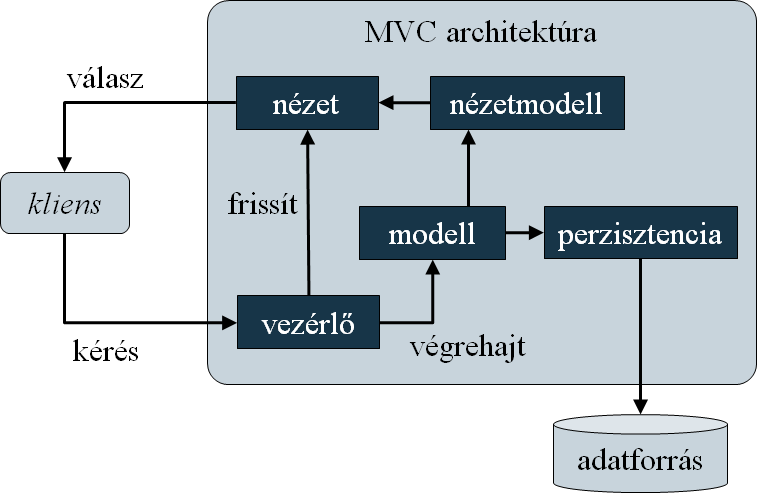
\includegraphics[width=1.0\textwidth]{developerguide/mvc-pattern}
	\caption{A Model-View-Controller architektúra}
	\label{fig:mvc-pattern}
\end{figure}
\begin{forest}
	for tree={
	  font=\ttfamily,
	  grow'=0,
	  child anchor=west,
	  parent anchor=south,
	  anchor=west,
	  calign=first,
	  edge path={
		\noexpand\path [draw, \forestoption{edge}]
		(!u.south west) +(7.5pt,0) |- node[fill,inner sep=1.25pt] {} (.child anchor)\forestoption{edge label};
	  },
	  before typesetting nodes={
		if n=1
		  {insert before={[,phantom]}}
		  {}
	  },
	  fit=band,
	  before computing xy={l=15pt},
	}
  [Views
	[Components/
	]
	[Features/
		  [AR/]
		  [Controls/]
		  [Info/]
	  [Screens/]
		  [Settings/]
		  [Slides/]
		  [User/]
	  ]
	  [ContentView.swift]
  ]
\end{forest}
\section{Hibakezelés és logolás}
\label{sec:error-handling-log}
Az alkalmazás a \emph{Serilog.Extensions.Logging.File} nyílt forráskódú programkönyvtár használatával valósítjuk meg \cite{SERILOG}. Az alkalmazás automatikusan logolja a futás közbeni eseményeket. A logolás beállításait az \emph{appsettings.json} (\ref{src:json} ábra) fájlban tudjuk személyreszabni. Az alábbi négy értéket írjuk felül az alkamazáshoz:
\begin{itemize}
	\item PathFormat: itt tudjuk megadni az alkalmazás logfájljainak a nevét és a mentési helyét. A \emph{\{Date\}} paraméter helyére az aktuális dátum kerül beillesztésre. Ha az elérési útban található mappa nem létezik azt a programkönyvtár automatikusan létrehozza a számunkra.
	\item OutputTemplate: itt adható meg a log üzenetek sablonja, hogy hogyan nézzenek ki a logolt üzenetek\footnote{Az \href{https://github.com/serilog/serilog/wiki/Formatting-Output}{alábbi linken} részletes leírást olvashatunk az \emph{OutputTemplate}-ben található paraméterek értékeiről.}.
	\item LogLevel: itt állíthatjuk be, hogy milyen minimum szintű események kerüljenek logolásra\cite{LogLevels}
\end{itemize}
\lstset{caption={appsettings.json}, label=src:json}
\begin{lstlisting}[language=json]
	...
	"Logging": {
		"PathFormat": "../Logs/log-{Date}.log",
		"OutputTemplate": "[{Timestamp:yyyy.MM.dd HH:mm:ss}] - [{Level:u}] - {Message}{NewLine}{Exception}",
		"LogLevel": {
		  "Default": "Debug",
		  "Microsoft": "Information"
		}
	},
	...
\end{lstlisting}
\section{Adatbázis}
\label{sec:database}
Az adatbázis
\section{Model réteg}
\label{sec:model}
\section{Vezérlő réteg}
\label{sec:controller}
\section{Nézet réteg}
\label{sec:view}